%%%%%%%%%%%%%%%%%%%%%%%%%%%%%%%%%%%%%%%%%%%%%%%%%%%%%%%%%%%%%%%%%%%%%
%                                                                   %
% NB: must be compiled with pdflatex -shell-escape poster_portrait  %
%                                                                   %
%%%%%%%%%%%%%%%%%%%%%%%%%%%%%%%%%%%%%%%%%%%%%%%%%%%%%%%%%%%%%%%%%%%%%

\documentclass[a0paper,portrait,fontscale=0.35]{baposter}

\usepackage{amsfonts,amsmath,amssymb}
\usepackage{graphicx,subcaption}

\usepackage{relsize}
\usepackage{natbib}
\usepackage{pgfplots}
\pgfplotsset{compat=1.9}
\pgfmathdeclarefunction{gauss}{2}{%
  \pgfmathparse{1/(#2*sqrt(2*pi))*exp(-((x-#1)^2)/(2*#2^2))}%
}


\usepackage{microtype}

\usepackage{environ}
\makeatletter
\newsavebox{\measure@tikzpicture}
\NewEnviron{scaletikzpicturetowidth}[1]{%
  \def\tikz@width{#1}%
  \def\tikzscale{1}\begin{lrbox}{\measure@tikzpicture}%
    \BODY
  \end{lrbox}%
  \pgfmathparse{#1/\wd\measure@tikzpicture}%
  \edef\tikzscale{\pgfmathresult}%
  \BODY
}
\makeatother


%%% Define a caption font
\newcommand{\mycaption}[1]{
  {
    \smaller
    \emph{#1}
  }
}

%%% Color Definitions %%%%%%%%%%%%%%%%%%%%%%%%%%%%%%%%%%%%%%%%%%%%%%%%%%%%%%%%%
\definecolor{oxford_blue}{RGB}{14,31,71}
\definecolor{oxford_border}{RGB}{14,31,71}

\begin{document}
\typeout{Poster rendering started}

\begin{poster}
  {
    % Show grid to help with alignment
    grid=false,
    columns=4,
    % Column spacing
    colspacing=0.7em,
    % Color style
    % headerColorOne=cyan!20!white!90!black,
    % borderColor=cyan!30!white!90!black,
    headerColorOne=oxford_blue,
    borderColor=oxford_border,
    headerFontColor=white,
    % Format of textbox
    textborder=faded,
    % Format of text header
    headerborder=open,
    headershape=roundedright,
    headershade=plain,
    background=none,
    bgColorOne=cyan!10!white,
    headerheight=0.08\textheight
  }
  % Eye Catcher: Oxford logo and personal picture
  {
    \makebox[0.23\textwidth]{
      \begin{tabular}{cc}
        
\includegraphics[height=0.05\textheight]{./img/oxlogo}
        &
          
\includegraphics[height=0.05\textheight]{./img/profile}
      \end{tabular}
      \hfill
    }
  }
  %%% Title %%%%%%%%%%%%%%%%%%%%%%%%%%%%%%%%%%%%%%%%%%%%%%%%%%%%%%%%%%%%%%%%%%%%%
  {\textsc{Pricing\,under\,uncertainty}}
  %%% Authors %%%%%%%%%%%%%%%%%%%%%%%%%%%%%%%%%%%%%%%%%%%%%%%%%%%%%%%%%%%%%%%%%%%
  {
    \vspace{0.5em}
    Asbj{\o}rn Nilsen Riseth ---
    % \texttt{riseth@maths.ox.ac.uk}\\[0.1em]
    \texttt{https://people.maths.ox.ac.uk/riseth}\\[0.1em]
    { Mathematical Institute, University of Oxford}
  }
  %%% InFoMM Logo %%%%%%%%%%%%%%%%%%%%%%%%%%%%%%%%%%%%%%%%%%%%%%%%%%%%%%%%%%%%%%%
  {
    \makebox[0.23\textwidth]{
      
\includegraphics[height=0.05\textheight]{./img/InFoMM}
    }
  }

  \headerbox{How do you decide the price of your products?}{name=introduction,span = 2,column=0,row=0}{
    Retail managers must decide the prices of hundreds of products
    to maximise revenue or profit.
    Such decisions must be made with only partial knowledge of future
    outcomes, which we will model as random variables.
    The industry is interested in understanding how to formulate
    optimisation problems with uncertainty, in particular the topics:
    \begin{itemize}
    \item Uncertainty in the objective --- how do we define optimality?
    \item Uncertainty in the constraint --- can we make sense of a
      ``random constraint''?
    \item Sequential decision problems --- how do we take into account
      the full value of each action?
    \end{itemize}


    We model the product demand per unit time $V(x)$ as a function of product
    price $x$. A discussion of the modelling aspect can be found in
    \citep{ryzin2012}. Define
    \begin{align}
      \mbox{Revenue}(x) &= xV(x),\\
      \mbox{Profit}(x,c) &= (x-c)V(x),& \text{given \emph{marginal cost} c}
    \end{align}

    One particular problem of industry interest is to
    understand how to handle the uncertainty of marginal costs in
    optimisation formulations.

    \vspace{1em}
    \begin{minipage}[c]{0.5\textwidth}
      \centering
      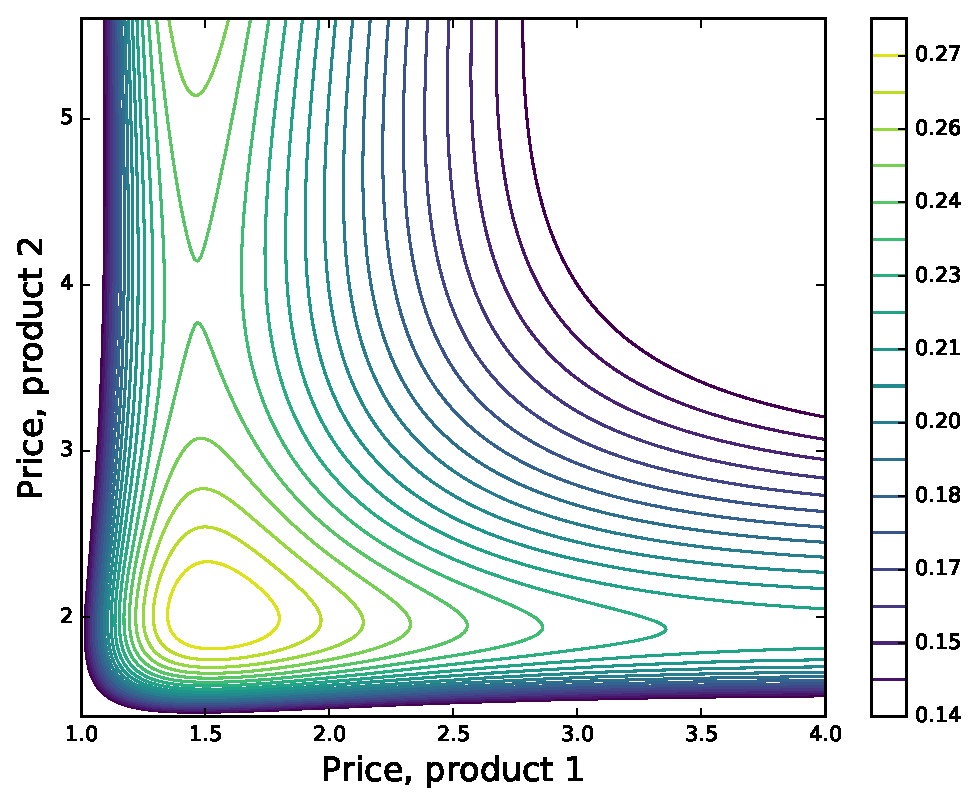
\includegraphics[width=0.9\textwidth]{./img/multiple_profit}\\
      \mycaption{Expected profit of two products}
    \end{minipage}%
    \begin{minipage}[c]{0.5\textwidth}
      \centering
      \begin{scaletikzpicturetowidth}{0.9\textwidth}
        \begin{tikzpicture}[inner sep=0.333em, outer
          sep=0.5\pgflinewidth, scale=\tikzscale]

          \begin{axis}[%[width=0.9\textwidth,
            grid=major,
            xmin=0.5,
            xmax=4,
            ymin=0,
            % title={Single product: Scale factor 1.0, elasticity -2.2},
            xlabel=Price,
            ylabel=Profit,
            domain=0.5:4,
            samples=100,
            % cycle list name=exotic,
            cycle list={
              {blue},
              {green},
              {red},
              {cyan},
              {purple}
            }
            ]
            \pgfplotsinvokeforeach {0.50,0.75,1.00,1.25,1.50}
            {
              \addplot+[mark=none] {(x-#1)*x^(-2.2)};
              \addlegendentry {$c=#1$};
            }
          \end{axis}
        \end{tikzpicture}
      \end{scaletikzpicturetowidth}
      \\
      \mycaption{\quad Profit depends on uncertain cost}
    \end{minipage}
  }

  \headerbox{Maximise uncertain profit}
  {name=randomobjective, column=0, below=introduction, above=bottom, span=2}
  {
    Take two prices which give rise
    to two different probabilistic forecasts of profit. How should a manager decide between
    the two prices? With the distributional information of the two competing choices,
    they can compare the possible outcomes.
    Our goal is to model the result of such a comparison.

    \vspace{0.5em}
    \textbf{Expected utility theory:}
    The degree of preference of an outcome is modelled by a utility
    function $u:\mathbb R\to\mathbb R$. The best choice is one that
    has the highest average utility:
    \begin{align}
      x_1\preceq x_2 \Leftrightarrow
      \mathbb E_C[u(\mbox{Profit}(x_1,c))] \leq
      \mathbb E_C[u(\mbox{Profit}(x_2,c)].
    \end{align}
    This approach weighs all outcomes according to their degree of
    preference and how probable they are. Risk-aversion requires
    that $u$ is concave and increasing.

    \vspace{0.5em}
    \begin{minipage}{0.5\textwidth}
      \centering
      \begin{scaletikzpicturetowidth}{0.9\textwidth}
        \begin{tikzpicture}[inner sep=0.333em, outer
          sep=0.5\pgflinewidth, scale=\tikzscale]
          \begin{axis}[
            ymajorgrids,
            title={Risk-averse utility function},
            xlabel=Wealth,
            ylabel=Utility,
            domain=-1.5:1.5,
            samples=150,
            ]
            \addplot+[mark=none] {x}
            node[pos=0.8, pin={[black]180:Risk neutral}]{};
            \addplot+[mark=none] {1-exp(-x)}
            node[pos=0.3, pin={[black]-45:$u(x)=1-\mathrm{e}^{-x}$}] {};
          \end{axis}
        \end{tikzpicture}
      \end{scaletikzpicturetowidth}
      % \\
      % \mycaption{\quad Risk-averse utility}
    \end{minipage}%
    \begin{minipage}{0.5\textwidth}
      \centering
      \begin{scaletikzpicturetowidth}{0.9\textwidth}
        \begin{tikzpicture}[inner sep=0.333em, outer
          sep=0.5\pgflinewidth, scale=\tikzscale]
          \begin{axis}[
            ymin=0,
            title={Risk-aversion increases the optimal price},
            xlabel=Price,
            ylabel={Expected utility of profit},
            ]
            \addplot+[mark=none] table [y index = {1}] {./img/cara_comparison.dat}
            node [pos=0.8, pin={[black]-90:Risk neutral}] {};
            \addplot+[mark=none] table [y index = {2}] {./img/cara_comparison.dat}
            node [pos=0.9, pin={[black]-90:$u(x)=1-\mathrm{e}^{-x}$}] {};
          \end{axis}
        \end{tikzpicture}
      \end{scaletikzpicturetowidth}
      % \\
      % \mycaption{\quad Risk-aversion increases the optimal price}
    \end{minipage}%

    \vspace{1em}

    \textbf{Mean-deviation approach:}
    Maximising average outcomes give the highest returns over the long term.
    To stabilise the returns over the medium term, we can try to
    minimise the uncertainty modelled by a deviation measure $\mathbb
    D$:
    \begin{align}
      \mathbb E[\mbox{Profit}]
      \quad
      \text{versus}
      \quad
      \mathbb D[\mbox{Profit}].
    \end{align}
    The measure can for example be the standard deviation, higher-order
    moments or the lower semi-deviation.
    The \emph{efficient frontier} shows what optimal trade-offs
    that can be made between such competing objectives.

    \vspace{0.5em}

    \begin{minipage}{0.5\textwidth}
      \centering
      \begin{scaletikzpicturetowidth}{0.9\textwidth}
        \begin{tikzpicture}[inner sep=0.333em, outer
          sep=0.5\pgflinewidth, scale=\tikzscale]
          \begin{axis}[
            xlabel=Standard deviation,
            ylabel=Expected profit,
            title = {Efficient frontier},
            scaled ticks = false,
            xticklabel style={
              /pgf/number format/precision=3,
              /pgf/number format/fixed,
              % /pgf/number format/fixed zerofill,
            }]
            \addplot[blue] table
            {./img/pareto_std_prof_2_nbi.dat};
            \draw [red, fill=red] (axis
            cs:.0799910964395231,.6358717068204365)
            circle (0.5mm) node[right, outer sep=1.5mm, text=black] {1};
            \draw [red, fill=red]
            (axis cs:.0856843689227338,.6554090852072043)
            circle (0.5mm) node[below, outer sep=1.5mm, text=black] {2};
            \draw [red, fill=red]
            (axis cs:.09725857996956377,.6590558821252489)
            circle (0.5mm) node[below, outer sep=1.5mm, text=black] {3};
          \end{axis}
        \end{tikzpicture}
      \end{scaletikzpicturetowidth}
    \end{minipage}%
    \begin{minipage}{0.5\textwidth}
      \centering
      \begin{scaletikzpicturetowidth}{0.9\textwidth}
        \begin{tikzpicture}[inner sep=0.333em, outer
          sep=0.5\pgflinewidth, scale=\tikzscale]
          \begin{axis}[
            % grid=major,
            xlabel=Profit,
            ylabel=Density,
            title={Gaussian approximations from frontier},
            xmin=0.3,
            xmax=1,
            domain=0.3:1,
            samples=150,
            ]
            \addplot+[mark=none]
            {gauss(.6358717068204365,.0799910964395231)};
            \addplot+[mark=none] {gauss(.6554090852072043,.0856843689227338)};
            \addplot+[mark=none]
            {gauss(.6590558821252489,.09725857996956377)};
            \legend {1,2,3};
          \end{axis}
        \end{tikzpicture}
      \end{scaletikzpicturetowidth}
    \end{minipage}

    \vspace{0.5em}
    We have created a software to automate the generation of the
    efficient frontier, available at
    \texttt{https://github.com/anriseth/MultiJuMP.jl}.
  }

  \headerbox{Further work}
  {name=furtherwork, column=2, row=0, span=2}
  {
    \textbf{Sequential decision problem:}
    How should we price a product to get rid of stock before a given
    time, e.g.~at an end-of-season sale?
    The goal will be to maximise revenue and minimise cost from unsold
    stock.
    A natural approach is to set a price for a time period with
    sales forecast $V_t$, then see
    how many products $\hat{V}_t$ are sold, and update the price accordingly.
    \begin{center}
      \begin{scaletikzpicturetowidth}{0.9\textwidth}
        \tikzstyle{init} = [pin edge={to-,thin,black}]
        \tikzstyle{state} = [draw, rectangle, rounded corners, fill=blue!20!white!90!black]
        \tikzstyle{value} = [draw, circle, fill=cyan!30!white!90!black]
        \tikzstyle{optim} = [draw, rectangle, fill=red!20]

        \begin{tikzpicture}[inner sep=0.333em, outer
          sep=0.5\pgflinewidth, scale=\tikzscale,
          node distance=2.5cm,auto,>=latex]
          \node [optim, align=center] (start) {Decision\\policy $X^\pi$};
          \node [pin={[init]above:$\hat{V}_1$}] (v0) [right of=start,
          node distance=2.7cm, state]
          {$V_1,\hat{V}_1$};
          \node [pin={[init]above:$\hat{V}_2$}] (v1)
          [right of=v0, node distance=3.3cm, state]
          {$V_2,\hat{V}_2$};
          \node (vt) [right of=v1, node distance=2.2cm] {...};
          \node [pin={[init]above:$\hat{V}_T$}] (vT)
          [right of=vt, node distance=2.2cm, state]
          {$V_T,\hat{V}_T$};

          \node (c0) [below of=v0, node distance=1.5cm, value]
          {$x_1\hat{V}_1$};
          \node (c1) [below of=v1, node distance=1.5cm, value] {$x_2\hat{V}_2$};
          \node (cT) [below of=vT, node distance=1.5cm, value, align=center] {$x_T\hat{V}_T$,\\$\hat{V}_T$};

          \node (totval) [below of=c1, node distance=2cm, optim] {Total value};


          \path[->] (start) edge node {$X_1^\pi$} (v0);
          \path[->] (v0) edge node {$X_2^\pi(V_1,\hat{V}_1)$} (v1);
          \path[->] (v1) edge node {$X_3^\pi$} (vt);
          \path[->] (vt) edge node {$X_{T}^\pi$} (vT);
          \path[-] (c0) edge (v0);
          \path[-] (c1) edge (v1);
          \path[-] (cT) edge (vT);

          \path[->] (c0) edge node [left, outer sep=2mm] {$u_1$} (totval);
          \path[->] (c1) edge node [right] {$u_2$} (totval);
          \path[->] (cT) edge node [right, outer sep=3mm] {$u_T$} (totval);

          \path[<->] (start) edge [bend right=30] node [left, outer sep=2mm] {Optimise} (totval);
        \end{tikzpicture}
      \end{scaletikzpicturetowidth}
      % \\
      % \mycaption{The sequential decision problem.}
    \end{center}
    The optimisation problem can be formulated as
    \begin{align}
      \max_{\pi\in \Pi}\{\mathbb E_{V} \sum_{t=1}^T u_t(x_t,V_t)\mid x_t
      = X_t^\pi(V_{t-1},\hat{V}_{t-1})\}.
    \end{align}

    \vspace{-0.1em}
    This can be computationally intractable. The challenge is to understand
    what policy-approximations that can be made in order to solve the problem.
    We will start by considering
    the approaches from \citep{powell2007approximate}.

    \vspace{-0.1em}
    \hrulefill

    \textbf{Optimisation of integral-forms:} Define a decision space $\mathcal X$, a parameter space
    $\mathcal Y$ and an objective $f:\mathcal X\times\mathcal Y\to
    \mathbb R$.
    Assume a probability density $\tau$ on $\mathcal Y$ and a utility
    function $u$ are given. We are interested in solving the problem
    \begin{align}
      \max_{x\in\mathcal X}\{\mathbb E_\tau [u(f(x,\cdot))]\}.
    \end{align}
    In retail, the dimension of $\mathcal Y$ can be on the order of
    hundreds. The expectation is therefore a high-dimensional integral
    that is expensive to approximate. The challenge is to design
    an algorithm to efficiently solve optimisations of
    integral-forms. Some points we would like to consider are:
    \begin{itemize}
    \item The structure of the integrand and domain can be important;
      we start to investigate cases with $f=\mbox{total profit}$ and
      $u(x)=1-e^{-x}$.
      % \item Optimality conditions such as Karush-Kuhn-Tucker.
    \item Gaussian Process interpolation, or Kriging, to approximate
      the integral.
    \item Build on the recently
      developed GLASSES algorithm \citep{gonzalez2015glasses}.
      The aim there is to achieve the best approximate
      solution for a given computational budget.
    \end{itemize}

  }

  \headerbox{Uncertainty in the constraint}
  {name=uncertainty, column=2, span=2, below=furtherwork}
  {
    Say a manager wants to maximise revenue, but keep his total profit
    above a given level $p_{min}$. In the deterministic approach one would
    impose a constraint on profit. With uncertainty one can only
    assert whether the price decision satisfied the constraint at a
    later date.
    A popular approach demands constraint satisfaction with
    some probability $\epsilon\in(0,1)$:
    \begin{align}
      \max_{x}\{\mbox{Revenue}(x)\mid
      \mathbb P(\mbox{Profit}(x,c)\geq p_{min})\geq \epsilon\}.
    \end{align}
    The two main problems with such an approach are that
    \begin{enumerate}
    \item it incurs implicit losses on revenue by restricting the
      feasible set;
    \item there is still a chance that the constraint is violated.
    \end{enumerate}
    Instead, one should investigate the trade-offs between objective and
    constraint as the feasible set is tightened.
    To model the managers trade-off decision one can penalise constraint
    violations in the mean or compare expected utilities.

    \vspace{0.5em}

    \begin{minipage}[h]{0.55\textwidth}
      \centering
      \begin{scaletikzpicturetowidth}{0.9\textwidth}
        \begin{tikzpicture}[inner sep=0.333em, outer
          sep=0.5\pgflinewidth, scale=\tikzscale]
          \begin{axis}[
            axis equal, view={0}{90},
            title={Compare objective and constraint distribution},
            xlabel=Profit $p$,
            ylabel=Revenue loss at $x^*$,
            colorbar,
            colorbar style={ylabel={Density of $p(x^*,C)$}}
            ]
            \addplot3[contour gnuplot={number=30,labels=false},mesh/ordering=y varies]
            table {./img/revloss_profdensity_lognormal.dat};
            \addplot[black,ultra thick] table
            {./img/revloss_quantile20_lognormal.dat};
            \addplot[black, dashed, thick] coordinates {(0.2,0.5) (0.2,0)}
            node[below]{$p_{min}$};
            \addplot[black, dashed, thick] coordinates {(0.47,0.42) (-0.08,0.42)}
            node[left, align=center]{Loss for\\$p_{min}=0.2$};
          \end{axis}
        \end{tikzpicture}
      \end{scaletikzpicturetowidth}
    \end{minipage}%
    \begin{minipage}[h]{0.45\textwidth}
      \centering
      \begin{scaletikzpicturetowidth}{0.97\textwidth}
        \begin{tikzpicture}[inner sep=0.333em, outer
          sep=0.5\pgflinewidth, scale=\tikzscale]
          \begin{axis}[
            title=Incorporate profit in objective to optimise trade-off,
            xlabel=Price $x$,
            ylabel=Mean total value,
            ]
            \addplot[thick, blue] table {./img/meantotal.dat}
            node[pos=0.8, text=black,pin={[black]-120:$r(x)-\frac{3}{2}\mathbb
              E_C(p_{min}-p(x,C))^+$}] {};
            \draw [red, fill=red] (axis cs:.707181019207018,1.1585660852991877) circle (1mm)
            node[right, outer sep=3mm, text=black] {Optimum trade-off};
          \end{axis}
        \end{tikzpicture}
      \end{scaletikzpicturetowidth}
    \end{minipage}%
    \vspace{-0.5em}
  }


  \headerbox{Acknowledgements}
  {name=acknowledgements, column=3, below=uncertainty, above=bottom, span=1}
  {
    \vspace{1em}
    \begin{center}
      
\includegraphics[width=0.65\textwidth]{./img/company_logo.eps}\\[1.5em]
      
\includegraphics[width=0.65\textwidth]{./img/epsrc_logo.eps}
    \end{center}
  }

  \headerbox{References}
  {name=references, column=2, below=uncertainty, above=bottom, span=1}
  {
    \smaller                                  % Make the whole text smaller
    \bibliographystyle{abbrv}                 % Use plain style
    \renewcommand{\section}[2]{\vspace{0.05em}} % Omit "References" title
    \bibliography{references}
  }

\end{poster}
\end{document}

%%% Local Variables:
%%% mode: latex
%%% TeX-master: t
%%% End:
